\documentclass[12pt,a4paper]{article}
\usepackage[utf8]{}
\usepackage{amsmath}
\usepackage{amsfonts}
\usepackage{xcolor}
\usepackage{titlesec}
\usepackage{mdframed}
\usepackage[english]{babel}
\usepackage{amssymb}
\usepackage{pgf,tikz,pgfplots}
\usepackage{graphicx}
\graphicspath{ {figures/} }
\usepackage{array}
\usepackage{cases}
\usepackage{listings}
\usepackage{color}
\usepackage{float} 
\usepackage{array, caption, tabularx,  ragged2e,  booktabs}
\usepackage{hyperref}
\usepackage{tabulary}
%\usepackage{minitoc}
\pgfplotsset{compat=1.5}
\usepackage{mathrsfs}
\usetikzlibrary{arrows, calc}
\usepackage{fancyhdr}
\pagestyle{fancy}
\usepackage[labelsep=endash]{caption}
\pagestyle{empty}
\definecolor{dkgreen}{rgb}{0,0.6,0}
\definecolor{gray}{rgb}{0.5,0.5,0.5}
\definecolor{mauve}{rgb}{0.58,0,0.82}
\lstset{frame=tb,
  language=C++,
  aboveskip=3mm,
  belowskip=3mm,
  showstringspaces=false,
  columns=flexible,
  basicstyle={\small\ttfamily},
  numbers=none,
  numberstyle=\tiny\color{gray},
  keywordstyle=\color{blue},
  commentstyle=\color{dkgreen},
  stringstyle=\color{mauve},
  breaklines=true,
  breakatwhitespace=true,
  tabsize=3
}
\renewcommand{\listfigurename}{Figures}
\renewcommand{\listtablename}{Tables}
\newcommand{\tabitem}{~~\llap{\textbullet}~~}
\usepackage[left=2cm,right=2cm,top=2cm,bottom=2cm]{geometry}
\author{Nguyễn Văn Lộc}
\newmdenv[linecolor=black,skipabove=\topsep,skipbelow=\topsep,
leftmargin=-5pt,rightmargin=-5pt,
innerleftmargin=5pt,innerrightmargin=5pt]{mybox}
\begin{document}
\fancyhf{}
\lhead{Lab 3: Sorting}
\chead{}
\rhead{20120131 - Nguyen Van Loc}
\cfoot{\thepage}
\rfoot{}
\lfoot{}
\pagestyle{fancy}
\renewcommand{\headrulewidth}{0pt}
\renewcommand{\footrulewidth}{0pt}
\begin{titlepage}
\begin{mybox}
\begin{center}
\fontsize{12}{12}\selectfont
\textbf{VIETNAM NATIONAL UNIVERSITY HO CHI MINH CITY}\\
\textbf{UNIVERSITY OF SCIENCE}\\
\textbf{FACULTY OF INFORMATION TECHNOLOGY}
\end{center}
\vskip 2 cm
\begin{figure}[H]
\begin{center}

\includegraphics[scale=0.25]{logo}
\end{center}
\end{figure}
\vskip 2 cm
\begin{center}
\fontsize{18}{14}\selectfont
\textbf{REPORT FOR LAB 3: SORTING}\\
\vskip 0.5 cm
\fontsize{20}{16}\selectfont
\textbf{DATA STRUCTURES AND ALGORITHMS}\\
\vskip 0.5 cm
\fontsize{18}{12}\selectfont
\textbf{TOPIC: SORTING ALGORITHMS}
\end{center}
\vskip 2 cm
\fontsize{14}{12}\selectfont
\textbf{Lecturer:} Doctor Nguyen Thanh Phuong\\
\textbf{Teaching Assisstant:} Master Bui Huy Thong\\
\textbf{Project Instructor:} Master Bui Huy Thong\\
\textbf{Class:} 20CTT1TN\\
\textbf{Student:} 20120131 \(-\) Nguyen Van Loc
\vskip 4 cm
\begin{center}
\textbf{HO CHI MINH CITY, NOVEMBER 2021}
\end{center}
\end{mybox}
\end{titlepage}
\section{Information page}
\textbf{Name:} Nguyen Van Loc\\
\textbf{Student ID:} 20120131\\
\textbf{Class:} 20CTT1TN\\
\textbf{Subject:} Data structures and algorithms\\
\textbf{Lecturer:} Doctor Nguyen Thanh Phuong\\
\textbf{Teaching Assisstant:} Master Bui Huy Thong\\
\textbf{Project Instructor:} Master Bui Huy Thong\\
\textbf{Topic:} Sorting algorithms

\newpage

\section{Introduction page}
I have completed 11/11 required algorithms, including: selection sort, insertion sort, bubble sort, shaker sort, shell sort, heap sort, merge sort, quick sort, counting sort, radix sort, and flash sort\\
For output specifications, I have completed 5/5 commands, 3 for algorithm mode and 2 for comparison mode.\\
Below is the hardware specifications of the computer I used to run these algorithms:
\begin{figure}[H]
\begin{center}
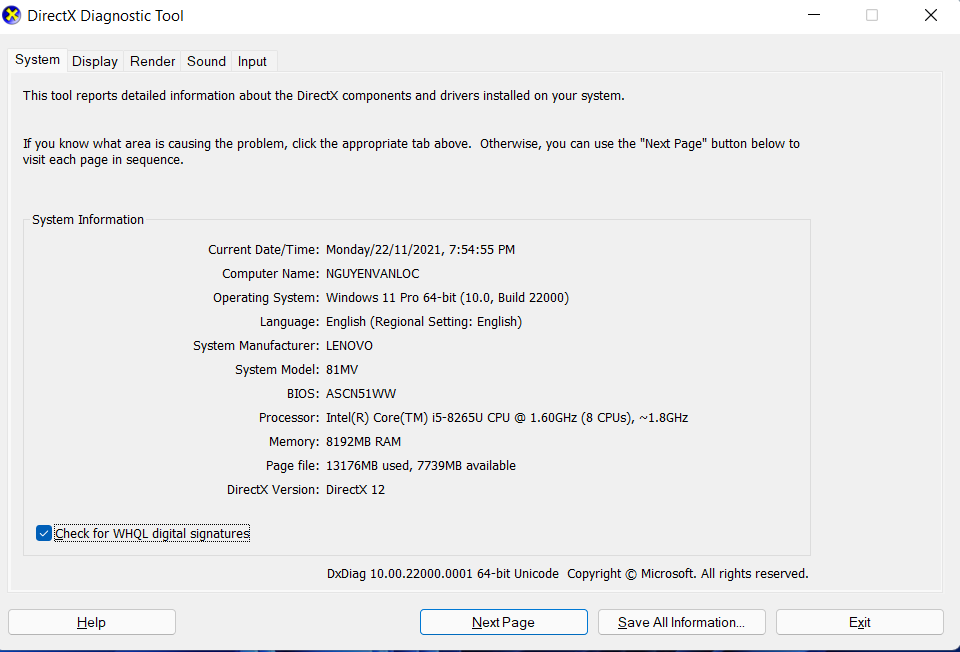
\includegraphics[scale=0.75]{hardware}
\end{center}
\caption{Hardware specifications}
\end{figure}

\newpage

\tableofcontents

\listoffigures
\listoftables
\addcontentsline{toc}{section}{tings}\renewcommand{\lstlistingname}{Code}
\renewcommand{\lstlistlistingname}{List of \lstlistingname s}
\lstlistoflistings

\newpage

\section{Algorithm presentation}
In this section, I will present the algorithms implemented in the project: ideas, step-by-step descriptions, and complexity evaluations. Varians/improvements of an algorithm, if there is any, will be also mentioned.\\
In this project, sorting algorithms are only used to sort the array in ascending order. Sorting in descending order will be similar.\\
Most of pseudocodes in this section will be presented in Pascal, with the 1-base array.
\subsection{Selection sort}
Selection sort is one of the simplest sorting algorithms.\\
Basic ideas of this algorithm is as followed:
\begin{itemize}
	\item In the first turn, choose  the minimum element in a[1..n], then swap it with a[1], that means a[1] becomes the minimum element of the array.
	\item In the second turn, choose the minimum element in a[2..n], then swap it with a[2], so that a[2] becomes the second lowest element of the array.
	\item ...
	\item In the i-th turn, choose the minimum in a[i..n], then swap it with a[i].
	\item In the (n-1)-th turn, choose the lower between a[n - 1] and a[n], then swap it with a[n-1].
\end{itemize}
\textbf{Pseudocodes}: \cite{gtvlt}
\lstset{language=Pascal} 
\begin{lstlisting}[caption = {Selection sort}]
begin
	for i := 1 to  n - 1 do
	begin
		jmin := i;
		for j := i + 1 to n do
			if (a[j] < a[jmin]) then jmin := j;
		if (jmin != i) then swap(a[jmin], a[i]);
	end
end
\end{lstlisting}
\textbf{Time complexity:} \cite{sscomp}
\begin{itemize}
\item Worst case: $O \left( {n^2} \right).$
\item Best case: $O \left( {n^2} \right).$
\item Average case: $O \left( {n^2} \right).$
\end{itemize}
\textbf{Space complexity:} $O \left( 1 \right).$ \cite{sscomp}

\subsection{Insertion sort}
\textbf{Ideas:} Consider the array a[1..n].\\
We see that the subarray with only one element a[1] can be seen as sorted.\\
Consider a[2], we compare it with a[1], if a[2] < a[1], we insert it before a[1].\\
With a[3], we compare it with the sorted subarray a[1..2], find the position to insert a[3] to that subarray to have an ascending order.\\
In a general speech, we will sort the array a[1..k] if the array a[1..k - 1] is already sorted by inserting a[k] to the appopriate position.\\
\textbf{Pseudocodes}: \cite{gtvlt}
\lstset{language=Pascal} 
\begin{lstlisting}[caption = {Insertion sort}]
begin
	for i := 2 to n do
	begin
		temp := a[i];
		j := i - 1;
		while (j > 0) and (temp < a[j]) do
		begin
			a[j + 1] = a[j];
			dec(j);
		end
		a[j + 1] = temp;
	end
end
\end{lstlisting}
\textbf{Time complexity: } \cite{comp}
\begin{itemize}
\item Worst case: $O \left( {n^2} \right).$
\item Best case: $O \left( {n} \right),$ in case the array is already sorted.
\item Average case: $O \left( {n^2} \right).$
\end{itemize}
\textbf{Space complexity:} $O \left( {1} \right).$ \cite{comp}\\
\textbf{Improvements:}
\begin{itemize}
\item Binary insertion sort $-$ find the position to insert using binary search, which reduces the number of comparisons. Details at link: \cite{bininsert}.
\item Another improvement of insertion sort is shell sort, which will be presented in section \ref{shellsort}
\end{itemize}

\subsection{Bubble sort}
\textbf{Ideas:} Bubble sort is the simples sorting algorithm, which swaps the adjacent elements if they are in wrong order, repeatedly $n$ times.\\
After the $i-$th turn, the $i-$th smallest element will be swapped to position $i.$\\
\textbf{Pseudocodes:} \cite{gtvlt}
\lstset{language=Pascal} 
\begin{lstlisting}[caption = {Bubble sort}]
begin
	for i := 2 to n do
		for j := n downto i do
		if (a[j - 1] > a[j]) then swap(a[j - 1], a[j]);
end
\end{lstlisting}
\textbf{Time complexity:} $O \left( {n^2} \right),$ not mentioned how the input data is. \cite{gtvlt}\\
\textbf{Space complexity:} $O \left( {1} \right).$ \cite{comp}\\
\textbf{Variations:} There are some variations in the implementation.
\begin{itemize}
\item Instead of top-down with \lstinline{j}, we can iterate from the bottom up, from \lstinline{i + 1} to \lstinline{n}.
\item Another variation is \lstinline{j} iterates from \lstinline{1} to \lstinline{n - i}. This is the version that I choose in my project.
\end{itemize}
\textbf{Improvements:} An improvement of bubble sort is shaker sort, which we will research in section \ref{shakersort}.

\subsection{Shaker sort (Cocktail sort)}
\label{shakersort}
\textbf{Ideas:} 
Shaker sort, also called cocktail sort or bi-directional bubble sort, is an improvement of bubble sort. In bubble sort, elements are traversed from left to right, i.e. in one direction only. But shaker sort will traverse in both direction, from left to right and from right to left, alternatively. \cite{shaker}\\
\textbf{Pseudocode:} \cite{thayP}
\lstset{language=Pascal} 
\begin{lstlisting}[caption = {Shaker sort}]
begin
	left := 2;
	right := n;
	k := n;
	repeat
	begin
		for j := right downto left do
			if (a[j - 1] > a[j]) then
			begin
				swap(a[j - 1], a[j]);
				k = j;
			end
		left = k + 1; //the last swap position
		for j := left to right do
			if (a[j - 1] > a[j]) then
			begin
				swap(a[j - 1], a[j]);
				k = j;
			end
		right = k - 1;
	end 
	
	until left > right;
	
end
\end{lstlisting}
\textbf{Time complexity:} \cite{shaksort}
\begin{itemize}
\item Worst case: $O \left( {n^2} \right).$
\item Best case: $O \left( {n} \right),$ in case the array is already sorted.
\item Average case: $O \left( {n^2} \right).$
\end{itemize}
\textbf{Space complexity:} $O \left( {1} \right).$ \cite{shaksort}

\subsection{Shell sort}
\label{shellsort}
A drawback of insertion sort is that we always have to insert an element to a position near the beginning of the array. In that case, we use shell sort.\\
\textbf{Ideas:} Consider an array a[1..n]. For an integer $h:$ $1 \leqslant h \leqslant n,$ we can divide the array into $h$ subarrays:
\begin{itemize}
\item Subarray 1: a[1], a[1 + h], a[1 + 2h]...
\item Subarray 2: a[2], a[2 + h], a[2 + 2h]...
\item ...
\item Subarray h: a[h], a[2h], a[3h] ...
\end{itemize}
Those subarrays are called subarrays with step $h.$ With a step $h,$ shell sort will use insertion sort for independent subarrays, then similarly with $\frac{h}{2}, \frac{h}{4}, ...$ until $h = 1.$\\
\textbf{Pseudocodes:}
\lstset{language=Pascal} 
\begin{lstlisting}[caption = {Shell sort}]
begin
	gap := n div 2;
	while (gap > 0) do
	begin
		for i := gap to n do
		begin
			j := i - gap;
			k := a[i];
			while (j > 0 and a[j] > k) do
			begin
				a[j + gap] := a[j];
				j = j - gap;
			end
			a[j + gap] := k;
		end	
		gap := gap div 2;
	end
end
\end{lstlisting}
\textbf{Time complexity:} \cite{shell}
\begin{itemize}
\item Worst case: $O \left( {n^2} \right).$
\item Best case: $O \left( {n \log n} \right).$
\item Average case: depends on the gap sequence.
\end{itemize}
\textbf{Space complexity:} $O \left( {1} \right).$ \cite{shell}

\subsection{Heap sort}
Heap sort was invented by J. W. J. Williams in 1981, this algorithm not only introduced an effective sorting algorithm but also built an important data structures to represent priority queues: heap data structure.
\subsubsection{Heap data structure}
Heap is a special binary tree. A binary tree is said to follow a heap data structure if:
\begin{itemize}
\item it is a complete binary tree,
\item all nodes in the tree satisfy that they are greater than their children, i.e. the greatest element is the root. Such a heap is called a max-heap. If instead, all nodes are smaller than their childen, it is called a min-heap. \cite{heap}
\end{itemize}
\begin{figure}[H]
\begin{center}
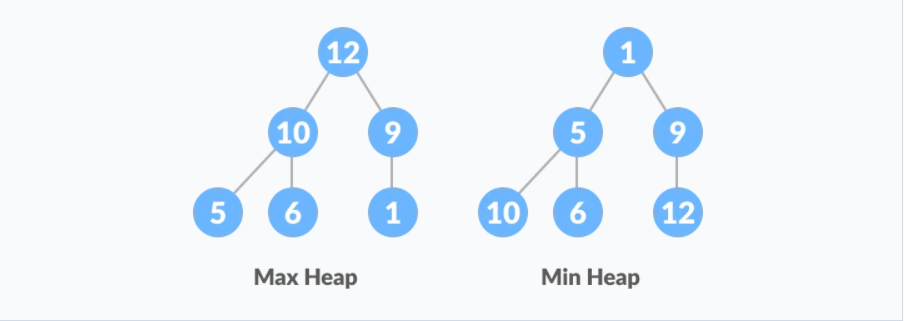
\includegraphics[scale=0.75]{heap}
\end{center}
\caption{Max-heap and min-heap. Source: \cite{heap}}
\end{figure}
\subsubsection{Build a min-heap}
To build a min heap, we: \cite{heapbuild}
\begin{itemize}
\item Create a new child node at the end of the heap (last level).
\item Add the new key to that node (append it to the array).
\item Move the child up until we reach the root node and the heap property is satisfied.
\end{itemize}
To remove/delete a root node in a min heap, we: \cite{heapbuild}
\begin{itemize}
\item Delete the root node.
\item Move the key of last child to root.
\item Compare the parent node with its children.
\item If the value of the parent is greater than its children, swap them, and repeat until the heap property is satisfied.
\end{itemize}
\subsubsection{Build a max-heap}
Building a max-heap is similar to building a min-heap.
\subsubsection{Pseudocodes}
\lstset{language=Pascal} 
\begin{lstlisting}[caption = {Heap sort}]
heapify(a[1..n], i)
begin
	max = i;
	left = 2 * i;
	right = 2 * i + 1;
	if (left <= n and a[left] > a[max]) then  max = left;
	if (right <= n and a[right] > a[max]) then max = right;
	if (max != i) then 
	begin
		swap(a[i], a[max]);
		heapify(a, n, max);
	end
end

heapsort(a[1..n])
begin
	for i := n div 2 - 1 downto 1 do heapify(a, i);
	for i := n downto 1 do 
	begin
		swap(a[0], a[i];
		heapify(a[1..i], 0)
	end
end
\end{lstlisting}
\textbf{Time complexity:} \cite{heap}
\begin{itemize}
\item Worst case: $O \left( {n \log n} \right).$
\item Best case: $O \left( {n \log n} \right).$
\item Average case: $O \left( {n \log n} \right).$
\end{itemize}
\textbf{Space complexity:} $O \left( {1} \right).$ \cite{heap}

\subsection{Merge sort}
Merge sort is a divide-and-conquer algorithm that was invented by John von Neumann in 1945. This is one of the most popular sorting algorithms. \\
\textbf{Ideas:} 
\begin{itemize}
\item Divide the array into two subarrays at the middle position.
\item Try to sort both subarrays, if we have not reached the base case yet, continue to divide them into subarrays.
\item Merge the sorted subarrays.
\end{itemize}
\textbf{Pseudocodes:}
\lstset{language=Pascal} 
\begin{lstlisting}[caption = {Merge sort}]
mergeSort(a[1..n])
begin
	if (n <= 1) do return;
	mid := n div 2;
	left[1..mid] := a[1..mid];
	right[1..n - mid] := a[mid + 1..n];
	
	mergeSort(left[1..mid]);
	mergeSort(right[1..n - mid]);
	
	i := 1; j := 1; k := 1;
	while (i <= mid and j <= n - mid)
	begin
		if (left[i] < right[j]) do 
		begin 
			a[k] := left[i];
			k := k + 1;
			i := i + 1;
		end 
		else 
		begin
			a[k] := right[j];
			k := k + 1;
			j := j + 1;
		end
	end
	while (i <= mid) do
	begin
		a[k] := left[i];
		k := k + 1;
		i := i + 1;	
	end
	while (j <= n - mid) do
	begin
		a[k] := right[j];
		k := k + 1;
		j := j + 1;
	end
end
\end{lstlisting}
\textbf{Time complexity:}  \cite{merge}
\begin{itemize}
\item Worst case: $O \left( {n \log n} \right).$
\item Best case: $O \left( {n \log n} \right).$
\item Average case: $O \left( {n \log n} \right).$
\end{itemize}
\textbf{Space complexity:} $O \left( {n} \right).$ \cite{merge}

\subsection{Quick sort}
Quicksort is a divide-and-conquer algorithm, introduced by C. A. R. Hoare, an English computer scientist, in 1960. It has become widely used due to its efficient, and is now one of the most popular sorting algorithms.\\
\textbf{Ideas:} \begin{itemize}
\item Sorting the array a[1..n] can be seen as sorting the segment from index $1$ to index $n$ of that array.
\item To sort a segment, if that segment has less than $2$ elements, then we have to do nothing, else we choose a random element to be the "pivot". All elements that are less than pivot will be arranged to a position before pivot, and all ones that are greater than pivot will be arranged to a position after pivot.
\item After that, the segment is divided into two segments, all elements in the first segment are less than pivot, and all elements in the second segment are greater than pivot. And now we have to sort two new segments, which have lengths smaller than the length of the initial segment.
\end{itemize}
In this project, I will choose the middle elements of the segments to be the pivot.\\
\textbf{Pseudocodes:} \cite{thayP}. 
\lstset{language=Pascal} 
\begin{lstlisting}[caption = {Quick sort}]
partition(a[1..n], l, r) 
begin
	mid := (l + r) div 2;
	pivot := a[mid];
	i := l - 1, j := r + 1;
	repeat 
		repeat
			inc(i);
		until (a[i] >= p);
		repeat
			dec(j);
		until (a[j] <= p)
		swap(a[i], a[j]);
	until (i >= j);
	swap(a[i], a[j]);
	swap(a[mid], a[j]);
	return j;
end

quicksort(a[1..n], l, r)
begin
	if (l < r) then
	begin
		s := partition(a, l, r);	
		quicksort(a, l, s - 1);
		quicksort(a, s + 1, r);
	end
end
\end{lstlisting}
\textbf{Time complexity:} \cite{quick}
\begin{itemize}
\item Worst case: $O \left( {n^2} \right).$
\item Best case: $O \left( {n \log n} \right).$
\item Average case: $O \left( {n \log n} \right).$
\end{itemize}
\textbf{Space complexity:} $O \left( {1} \right).$ \cite{quick}\\
\textbf{Variations:} Below is the implementation of quicksort using recursion. There is also an iterative algorithms, which can be found at: \cite{itequick} 

\subsection{Counting sort}
\label{countingsort}
Counting sort is a sorting algorithm working by counting the number of objects having distinct key values (a kind of hashing). \cite{count}\\
\textbf{Ideas:} Iterate through the input, count the number of times each item occurs, then use those results to calculate an item's index in the sorted array. \cite{counting}\\
This algorithm works when the array contains of nonnegative integers in range $\left[ {l, u} \right].$ The case that array is negative, the algorithms can also work but I will not mention it here.\\
\textbf{Pseudocodes:} \cite{thayP}
\lstset{language=Pascal} 
\begin{lstlisting}[caption = {Counting sort}]
countingsort(a[1..n])
begin
	f[0..u] := {0};
	for i:= 1 to n do inc(f[a[i]]);
	for i:= 1 to u do f[i] := f[i - 1] + f[i];
	//after this step, f[i] will be the number of elements that are less 
	than or equal to i.
	b[1..n];
	for i := n downto 1 do
	begin
		b[f[a[i]]] = a[i];
		dec(f[a[i]]);
	end
	a := b;
end
\end{lstlisting}
Counting sort works well when $n \approx u,$ but it will be "disastrous" if $u \gg n.$ \cite{thayP}\\
\textbf{Time complexity:} $O \left( {n + u} \right).$ \cite{count}\\
\textbf{Space complexity:} $O \left( {n + u} \right).$ \cite{count}

\subsection{Radix sort}
Like counting sort mentioned in section \ref{countingsort}, radix sort only works with integer.\\
\textbf{Ideas:} sort the array using counting sort (or any stable algorithms) according to the $i-$th digit. \cite{radix}\\
Let $d$ be the maximum number of digits of elements in the array, and $b$ be the base used to represent array, for example, for decimal system, $b = 10.$\\
\textbf{Pseudocodes:} \cite{thayP}
\lstset{language=Pascal} 
\begin{lstlisting}[caption = {Radix sort}]
sort(a[1..n], k)
begin
	f[0..b - 1] := {0};
	for i := 1 to n do inc(f[digit(a[i], k)]);
	for i := 1 to b - 1 to f[i] := f[i] + f[i - 1];
	b[1..n]
	for i := n downto 1 do
	begin
		j := digit(a[i], k);
		b[f[j]] = a[i];
		f[j]--;
	end
	a := b;
end

LSDradixsort(a[1..n], d)
begin
	for k := 0 to d do sort(a, k);
end
\end{lstlisting}
\textbf{Time complexity:} $O \left( {d \left( {n + b} \right)} \right).$ \cite{radix}\\
\textbf{Space complexity:} $O \left( n \right).$ \cite{radix}

\subsection{Flash sort}
Flash sort is a distribution sorting algorithm, which has the time complexity approxiamtely linear complexity. \cite{flash} Flash sort was invented by Dr. Neubert in 1997. He named the algorithm "flash" sort because he was confident that this algorithm is very fast.\\
\textbf{Ideas:} The algorithm is divided into three stages. \cite{thayP} \cite{flashsort}
\begin{itemize}
\item Stage 1: Classification of elements of the array. 
\item Stage 2: Partition of elements.
\item Stage 3: Sort the elements in each partition.
\end{itemize}
\subsubsection{Stage 1: Classification of elements of the array}
Let $m$ be the number of classes. The element $a_i$ will be in the $k-$th class with:
$${k_{{a_i}}} = \left\lfloor {\frac{{\left( {m - 1} \right)\left( {{a_i} - {{\min }_a}} \right)}}{{{{\max }_a} - {{\min }_a}}}} \right\rfloor + 1.$$
\textbf{Pseudocodes:} \cite{thayP}
\lstset{language=Pascal} 
\begin{lstlisting}[caption = {Flash sort - stage 1}]
L[1..m] := {0};
for i := 1 to n do
begin
	k := (m - 1) * (a[i] - min) div (max - min);
	inc(L[k]);
end
for k:= 2 to n do
begin
	L[k] := L[k] + L[k - 1];
end
\end{lstlisting}
After this stage, \lstinline{L[k]} will point to the right boundary of the $k-$th class.
\subsubsection{Stage 2: Partition of elements}
The elements are sorted by \textit{in situ permutation.} During the permutation, the \lstinline{L[k]} are decremented by a unit step at each new placement of an element of class $k.$ A crucial aspect of this algorithm is identifying new cycle leaders. A cycle ends, if the vector \lstinline{L[k]} points to the position of an element below boundary of class $k.$ The new cycle leader is the element situated in the lowest position complying to the complimentary condition, i.e. for which \lstinline{L[k]} points to a position with $i \leqslant {L_{{k_{{a_i}}}}}.$ \cite{flashsort}\\
\textbf{Psedocodes:} \cite{thayP}
\lstset{language=Pascal} 
\begin{lstlisting}[caption = {Flash sort - stage 2}]
count := 1;
i := 1;
k := m;
while (count <= n) do
begin
	while (i > L[k]) do
	begin
		inc(i);
		k := (m - 1) * (a[i] - min) div (max - min) + 1;
	end
	x := a[i];
	while (i <= L[k]) do
	begin
		k := (m - 1) * (x - min) div (max - min) + 1;
		y := a[L[k]];
		a[L[k]] := x;
		x := y;
		dec(L[k]);
		inc(count);
	end
end
\end{lstlisting}
\subsubsection{Stage 3: Sort the elements in each partition}
A small number of partially distinguishable elements are sorted locally within their classes either by recursion or by a simple conventional sort algorithm. \cite{flashsort}\\
In this project, I will choose insertion sort for this stage.\\
\textbf{Psedocodes:} \cite{thayP}
\lstset{language=Pascal} 
\begin{lstlisting}[caption = {Flash sort - stage 3}]
for k := 2 to m do
begin
	for i := L[k] - 1 to L[k - 1] do
	begin
		if (a[i] > a[i + 1]) then
		begin
			t := a[i];
			j := i;
			while (t > a[j + 1]) do
			begin
				a[j] := a[j + 1;
				inc(j);
			end
			a[j] := t;
		end
	end
end
\end{lstlisting}
This code is written correctly because the last class only contains of maximum element of the array, therefore it has been already sorted.
\subsubsection{Complexity}
\textbf{Time complexity:} $O \left( {\frac{n^2}{m}} \right).$\\
Experiments has shown that $m \approx 0.43n$ will be the best for this algorithm. In that case, time complexity of the algorithm is linear. \cite{thayP}\\
\textbf{Space complexity:} $O \left( m \right).$

\newpage

\section{Experimental results and comments}
\subsection{Tables of running time and comparisons count}
\noindent\setlength\tabcolsep{3pt}%
\begin{center}
\begin{table}[H]
\begin{tabulary}{0.7\textwidth}{|c|c|c|c|c|c|c|}
\hline 
\multicolumn{7}{c}{Data order: Randomized}\\ 
\hline 
Data size & \multicolumn{2}{c}{10000}& \multicolumn{2}{c}{30000}  &  \multicolumn{2}{c}{50000}  \\ 
\hline 
Resulting statics & Running time & Comparisons & Running time & Comparisons & Running time & Comparisons \\ 
\hline 
Selection sort & 0.125588 & 100019998 & 1.02347 & 90059998 & 2.81835 & 2500099998 \\ 
\hline 
Insertion sort & 0.060877 & 50096183 & 0.53271 & 452071438 & 1.46487 & 1250497473 \\ 
\hline 
Bubble sort & 0.275781 & 100009999 & 2.70246 & 900029999 & 8.1757 & 2500049999 \\ 
\hline 
Shaker sort & 0.221612 & 66920546 & 2.01225 & 602416029 & 5.53941 & 1668740213 \\ 
\hline 
Shell sort & 0.001633 & 630438 & 0.00589 & 2331067 & 0.013429 & 4629303 \\ 
\hline 
Heap sort & 0.009767 & 89996 & 0.007112 & 269996 & 0.018274 & 449996 \\ 
\hline 
Merge sort & 0.003842 & 337226 & 0.010604 & 1104458 & 0.018144 & 1918922 \\ 
\hline 
Quick sort & 0.001064 & 268649 & 0.003564 & 918072 & 0.006575 & 1571763 \\ 
\hline 
Counting sort & 0.000272 & 50004 & 0.00088 & 150004 & 0.001899 & 250004 \\ 
\hline 
Radix sort & 0.000581 & 140058 & 0.003068 & 510072 & 0.00367 & 850072 \\ 
\hline 
Flash sort & 0.000342 & 98814 & 0.001074 & 301965 & 0.002341 & 479127 \\ 
\hline 
\end{tabulary}
\caption{Data order: Randomized - table 1}
\end{table}
\end{center}

\noindent\setlength\tabcolsep{3pt}%
\begin{center}
\begin{table}[H]
\begin{tabulary}{0.65\textwidth}{|c|c|c|c|c|c|c|}
\hline 
\multicolumn{7}{c}{Data order: Randomized}\\ 
\hline 
Data size & \multicolumn{2}{c}{100000}& \multicolumn{2}{c}{300000}  &  \multicolumn{2}{c}{500000}  \\ 
\hline 
Resulting statics & Running time & Comparisons & Running time & Comparisons & Running time & Comparisons \\ 
\hline 
Selection sort & 11.2068  & 10000199998 & 98.3619  & 90000599998 & 298.723  & 250000999998 \\
\hline 
Insertion sort & 5.781    & 5019075369  & 52.6586  & 44979677317 & 145.002  & 124933091986 \\
\hline 
Bubble sort    & 31.7843  & 10000099999 & 290.83   & 90000299999 & 805.643  & 250000499999 \\
\hline 
Shaker sort    & 22.3527  & 6684229390  & 203.353  & 59984439772 & 564.835  & 166525795318 \\
\hline 
Shell sort     & 0.025796 & 10033440    & 0.085129 & 36188397    & 0.153476 & 67911677     \\
\hline 
Heap sort      & 0.027132 & 899996      & 0.116084 & 2699996     & 0.179792 & 4499996      \\
\hline 
Merge sort     & 0.018512 & 4037850     & 0.060769 & 13051418    & 0.105907 & 22451418     \\
\hline 
Quick sort     & 0.013801 & 3302209     & 0.042058 & 10782282    & 0.073066 & 19032583     \\
\hline 
Counting sort  & 0.001915 & 500004      & 0.005841 & 1500004     & 0.012324 & 2500004      \\
\hline 
Radix sort     & 0.007252 & 1700072     & 0.025703 & 6000086     & 0.0458   & 10000086     \\
\hline 
Flash sort     & 0.00513  & 1019156     & 0.017335 & 3047744     & 0.036041 & 4843142  \\
\hline 
\end{tabulary}
\caption{Data order: Randomized - table 2}
\end{table}
\end{center}

\noindent\setlength\tabcolsep{3pt}%
\begin{center}
\begin{table}[H]
\begin{tabulary}{0.7\textwidth}{|c|c|c|c|c|c|c|}
\hline 
\multicolumn{7}{c}{Data order: Sorted}\\ 
\hline 
Data size & \multicolumn{2}{c}{10000}& \multicolumn{2}{c}{30000}  &  \multicolumn{2}{c}{50000}  \\ 
\hline 
Resulting statics & Running time & Comparisons & Running time & Comparisons & Running time & Comparisons \\ 
\hline 
Selection sort & 0.113015            & 100019998 & 1.00498             & 900059998 & 2.81835  & 2500099998 \\
\hline 
Insertion sort & $3.6 \cdot 10^{-5}$ & 29998     & 0.0001              & 89998     & 0.000169 & 149998   \\
\hline 
Bubble sort    & 0.114492            & 100009999 & 1.00117             & 900029999 & 2.77147   & 2500049999 \\
\hline 
Shaker sort    & $3 \cdot 10^{-5}$   & 20002     & $6.7 \cdot 10^{-5}$ & 60002     & 0.000445 & 100002     \\
\hline 
Shell sort     & 0.000429            & 360042    & 0.00177             & 1170050   & 0.002384 & 2100049    \\
\hline 
Heap sort      & 0.003071            & 89996     & 0.005536            & 269996    & 0.010559 & 449996     \\
\hline 
Merge sort     & 0.000969            & 337226    & 0.002866            & 1104458   & 0.009389 & 1918922    \\
\hline 
Quick sort     & 0.000245            & 154959    & 0.000815            & 501929    & 0.001504 & 913850     \\
\hline 
Counting sort  & 0.000188            & 50004     & 0.000448            & 150004    & 0.000998 & 250004     \\
\hline 
Radix sort     & 0.000579            & 140058    & 0.003068            & 510072    & 0.00367  & 850072     \\
\hline 
Flash sort     & 0.000286            & 127992    & 0.000863            & 383992    & 0.001465 & 639992   \\
\hline 
\end{tabulary}
\caption{Data order: Sorted - table 1}
\end{table}
\end{center}

\noindent\setlength\tabcolsep{3pt}%
\begin{center}
\begin{table}[H]
\begin{tabulary}{0.65\textwidth}{|c|c|c|c|c|c|c|}
\hline 
\multicolumn{7}{c}{Data order: Sorted}\\ 
\hline 
Data size & \multicolumn{2}{c}{100000}& \multicolumn{2}{c}{300000}  &  \multicolumn{2}{c}{500000}  \\ 
\hline 
Resulting statics & Running time & Comparisons & Running time & Comparisons & Running time & Comparisons \\ 
\hline 
Selection sort & 11.2068  & 10000199998 & 98.3619  & 90000599998 & 298.723  & 250000999998 \\
\hline 
Insertion sort & 0.000325 & 299998       & 0.00099  & 899998      & 0.001617 & 1499998      \\
\hline 
Bubble sort    & 11.0277  & 10000099999  & 102.55   & 90000299999 & 278.658  & 250000499999 \\
\hline 
Shaker sort    & 0.000561 & 200002       & 0.000648 & 600002      & 0.001081 & 1000002      \\
\hline 
Shell sort     & 0.005229 & 4500051      & 0.018094 & 15300061    & 0.030237 & 25500058     \\
\hline 
Heap sort      & 0.032474 & 899996       & 0.072256 & 2699996     & 0.121933 & 4499996      \\
\hline 
Merge sort     & 0.011628 & 4037850      & 0.034167 & 13051418    & 0.059151 & 22451418     \\
\hline 
Quick sort     & 0.003875 & 1927691      & 0.01214  & 6058228     & 0.017523 & 10310733     \\
\hline 
Counting sort  & 0.001403 & 500004       & 0.004284 & 1500004     & 0.007221 & 2500004      \\
\hline 
Radix sort     & 0.007746 & 1700072      & 0.030804 & 6000086     & 0.045303 & 10000086     \\
\hline 
Flash sort     & 0.002968 & 1279992      & 0.00882  & 3839992     & 0.014181 & 6399992     \\
\hline 
\end{tabulary}
\caption{Data order: Sorted - table 2}
\end{table}
\end{center}

\noindent\setlength\tabcolsep{3pt}%
\begin{center}
\begin{table}[H]
\begin{tabulary}{0.7\textwidth}{|c|c|c|c|c|c|c|}
\hline 
\multicolumn{7}{c}{Data order: Reversed}\\ 
\hline 
Data size & \multicolumn{2}{c}{10000}& \multicolumn{2}{c}{30000}  &  \multicolumn{2}{c}{50000}  \\ 
\hline 
Resulting statics & Running time & Comparisons & Running time & Comparisons & Running time & Comparisons \\ 
\hline 
Selection sort & 0.10871  & 100019998 & 0.959207 & 900059998 & 2.79584  & 2500099998 \\
\hline 
Insertion sort & 0.119653 & 100009999 & 1.04109  & 900029999 & 2.95031  & 2500049999 \\
\hline 
Bubble sort    & 0.261722 & 100009999 & 2.17328  & 900029999 & 6.11784  & 2500049999 \\
\hline 
Shaker sort    & 0.252528 & 100005001 & 2.24013  & 900015001 & 6.17515  & 2500025001 \\
\hline 
Shell sort     & 0.000561 & 475175    & 0.003068 & 1554051   & 0.003583 & 2844628    \\
\hline 
Heap sort      & 0.003353 & 89996     & 0.005536 & 269996    & 0.010559 & 449996     \\
\hline 
Merge sort     & 0.001244 & 337226    & 0.003341 & 1104458   & 0.00547  & 1918922    \\
\hline 
Quick sort     & 0.00028  & 164975    & 0.000948 & 531939    & 0.001639 & 963861     \\
\hline 
Counting sort  & 0.000137 & 50004     & 0.000929 & 150004    & 0.000998 & 250004     \\
\hline 
Radix sort     & 0.000598 & 140058    & 0.002213 & 510072    & 0.003443 & 850072     \\
\hline 
Flash sort     & 0.000267 & 110501    & 0.000806 & 331501    & 0.001302 & 552501  \\  
\hline 
\end{tabulary}
\caption{Data order: Reversed - table 1}
\end{table}
\end{center}

\noindent\setlength\tabcolsep{3pt}%
\begin{center}
\begin{table}[H]
\begin{tabulary}{0.7\textwidth}{|c|c|c|c|c|c|c|}
\hline 
\multicolumn{7}{c}{Data order: Reversed}\\ 
\hline 
Data size & \multicolumn{2}{c}{100000}& \multicolumn{2}{c}{300000}  &  \multicolumn{2}{c}{500000}  \\ 
\hline 
Resulting statics & Running time & Comparisons & Running time & Comparisons & Running time & Comparisons \\ 
\hline 
Selection sort & 10.7125  & 10000199998 & 95.9219  & 90000599998 & 267.031  & 250000999998 \\
\hline 
Insertion sort & 11.5629  & 10000099999 & 103.857  & 90000299999 & 291/045  & 250000499999 \\
\hline 
Bubble sort    & 24.4371  & 10000099999 & 221.602  & 90000299999 & 616.86   & 250000499999 \\
\hline 
Shaker sort    & 24.8658  & 10000050001 & 226.276  & 90000150001 & 628.922  & 250000250001 \\
\hline 
Shell sort     & 0.007358 & 6089190     & 0.023358 & 20001852    & 0.04012  & 33857581     \\
\hline 
Heap sort      & 0.021055 & 899996      & 0.068389 & 2699996     & 0.123764 & 4499996      \\
\hline 
Merge sort     & 0.011581 & 4037850     & 0.033862 & 13051418    & 0.058475 & 22451418     \\
\hline 
Quick sort     & 0.00334  & 2027703     & 0.01059  & 6358249     & 0.017891 & 10810747     \\
\hline 
Counting sort  & 0.001819 & 500004      & 0.0049   & 1500004     & 0.007136 & 2500004      \\
\hline 
Radix sort     & 0.007137 & 1700072     & 0.025565 & 6000086     & 0.042483 & 10000086     \\
\hline 
Flash sort     & 0.002797 & 1105001     & 0.009906 & 3315001     & 0.013324 & 5525001 \\
\hline 
\end{tabulary}
\caption{Data order: Reversed - table 2}
\end{table}
\end{center}

\noindent\setlength\tabcolsep{3pt}%
\begin{center}
\begin{table}[H]
\begin{tabulary}{0.7\textwidth}{|c|c|c|c|c|c|c|}
\hline 
\multicolumn{7}{c}{Data order: Nearly sorted}\\ 
\hline 
Data size & \multicolumn{2}{c}{10000}& \multicolumn{2}{c}{30000}  &  \multicolumn{2}{c}{50000}  \\ 
\hline 
Resulting statics & Running time & Comparisons & Running time & Comparisons & Running time & Comparisons \\ 
\hline
Selection sort & 0.114235 & 100019998 & 1.01536  & 900059998 & 2.79563  & 2500099998 \\
\hline 
Insertion sort & 0.00027  & 219622    & 0.000755 & 595570    & 0.001001 & 858990     \\
\hline 
Bubble sort    & 0.113966 & 100009999 & 0.98869  & 900029999 & 2.76097  & 2500049999 \\
\hline 
Shaker sort    & 0.000583 & 219726    & 0.001456 & 603170    & 0.001938 & 873634     \\
\hline 
Shell sort     & 0.000578 & 416560    & 0.00194  & 1321108   & 0.005379 & 2380925    \\
\hline 
Heap sort      & 0.002457 & 89996     & 0.00639  & 269996    & 0.011723 & 449996     \\
\hline 
Merge sort     & 0.001216 & 337226    & 0.004687 & 1104458   & 0.006034 & 1918922    \\
\hline 
Quick sort     & 0.000246 & 154999    & 0.000826 & 501973    & 0.001523 & 913898     \\
\hline 
Counting sort  & 0.000152 & 50004     & 0.00046  & 150004    & 0.000718 & 250004     \\
\hline 
Radix sort     & 0.000592 & 140058    & 0.002119 & 510072    & 0.003794 & 850072     \\
\hline 
Flash sort     & 0.000289 & 127968    & 0.000882 & 383962    & 0.001456 & 639962    \\
\hline 
\end{tabulary}
\caption{Data order: Nearly sorted - table 1}
\end{table}
\end{center}

\noindent\setlength\tabcolsep{3pt}%
\begin{center}
\begin{table}[H]
\begin{tabulary}{0.7\textwidth}{|c|c|c|c|c|c|c|}
\hline 
\multicolumn{7}{c}{Data order: Nearly sorted}\\ 
\hline 
Data size & \multicolumn{2}{c}{100000}& \multicolumn{2}{c}{300000}  &  \multicolumn{2}{c}{500000}  \\ 
\hline 
Resulting statics & Running time & Comparisons & Running time & Comparisons & Running time & Comparisons \\ 
\hline 
Selection sort & 11.5729  & 10000199998 & 97.5573  & 90000599998 & 278.073  & 250000999998 \\
\hline 
Insertion sort & 0.002272 & 1975946     & 0.005013 & 4436926     & 0.00916  & 8122834      \\
\hline 
Bubble sort    & 11.0646  & 10000099999 & 99.9988  & 90000299999 & 279.598  & 250000499999 \\
\hline 
Shaker sort    & 0.011098 & 1970942     & 0.009868 & 4527181     & 0.01822  & 8481121      \\
\hline 
Shell sort     & 0.008393 & 5163287     & 0.030022 & 16636275    & 0.035062 & 27752013     \\
\hline 
Heap sort      & 0.022278 & 899996      & 0.097582 & 2699996     & 0.121831 & 4499996      \\
\hline 
Merge sort     & 0.011873 & 4037850     & 0.033909 & 13051418    & 0.059821 & 22451418     \\
\hline 
Quick sort     & 0.003395 & 1927735     & 0.010117 & 6058260     & 0.017855 & 10310769     \\
\hline 
Counting sort  & 0.001416 & 500004      & 0.004279 & 1500004     & 0.008047 & 2500004      \\
\hline 
Radix sort     & 0.007354 & 1700072     & 0.025246 & 6000086     & 0.045863 & 10000086     \\
\hline 
Flash sort     & 0.003038 & 1279962     & 0.008703 & 3839958     & 0.014624 & 6399962     \\
\hline 
\end{tabulary}
\caption{Data order: Nearly sorted - table 2}
\end{table}
\end{center}

\subsection{Line graphs of running time}
\begin{center}
\begin{figure}[H]
\center{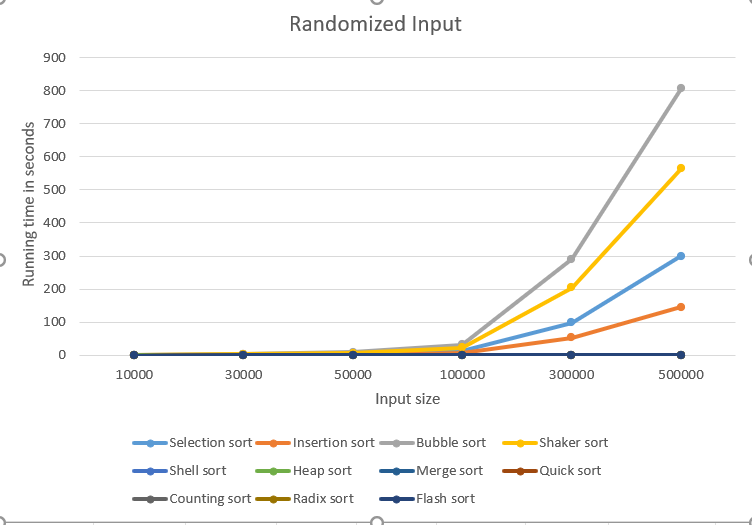
\includegraphics[scale=0.9]{LineGraph1}}
\caption{Line graph of running time for randomized input}
\end{figure}
\end{center}

\begin{center}
\begin{figure}[H]
\center{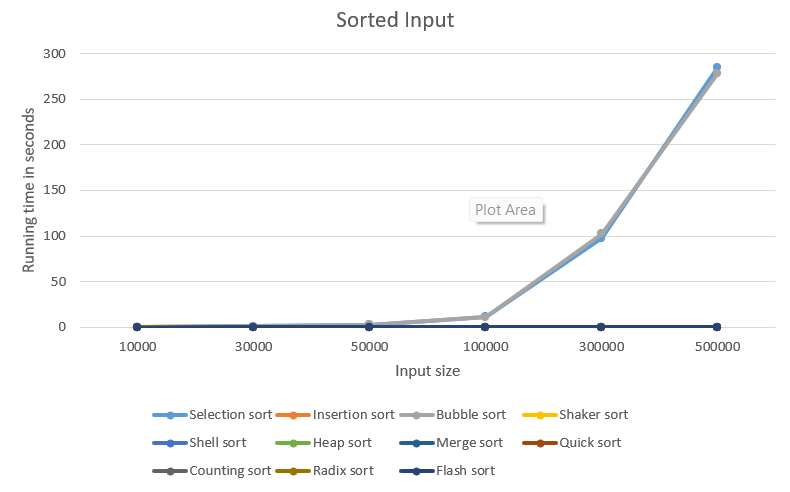
\includegraphics[scale=0.9]{LineGraph2}}
\caption{Line graph of running time for sorted input}
\end{figure}
\end{center}

\begin{center}
\begin{figure}[H]
\center{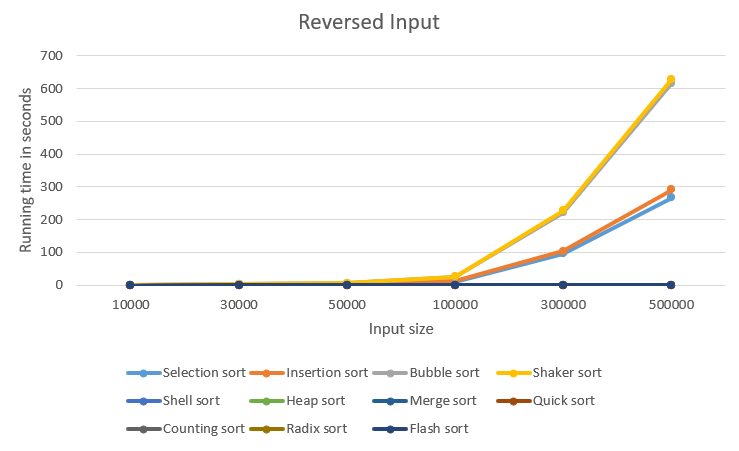
\includegraphics[scale=0.9]{LineGraph3}}
\caption{Line graph of running time for reversed input}
\end{figure}
\end{center}

\begin{center}
\begin{figure}[H]
\center{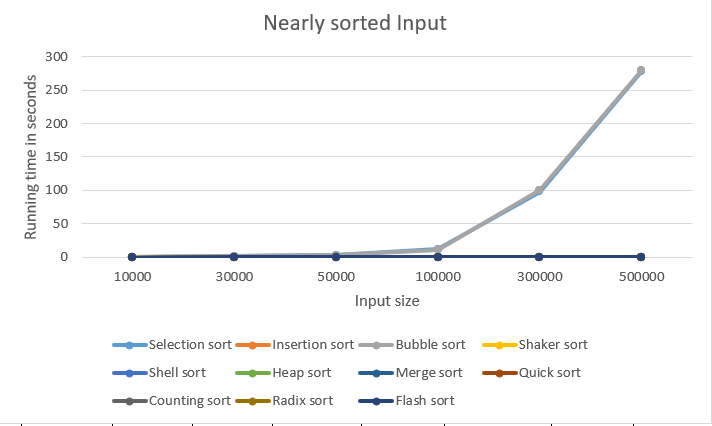
\includegraphics[scale=0.9]{LineGraph4}}
\caption{Line graph of running time for nearly sorted input}
\end{figure}
\end{center}

\subsection{Bar charts of comparisons}
\begin{center}
\begin{figure}[H]
\center{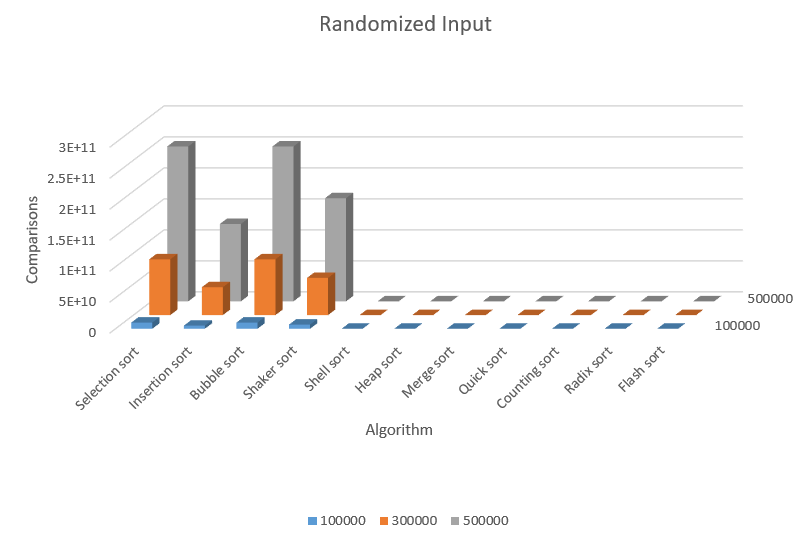
\includegraphics[scale=0.9]{BarChart1}}
\caption{Bar chart of comparisons for randomized input}
\end{figure}
\end{center}

\begin{center}
\begin{figure}[H]
\center{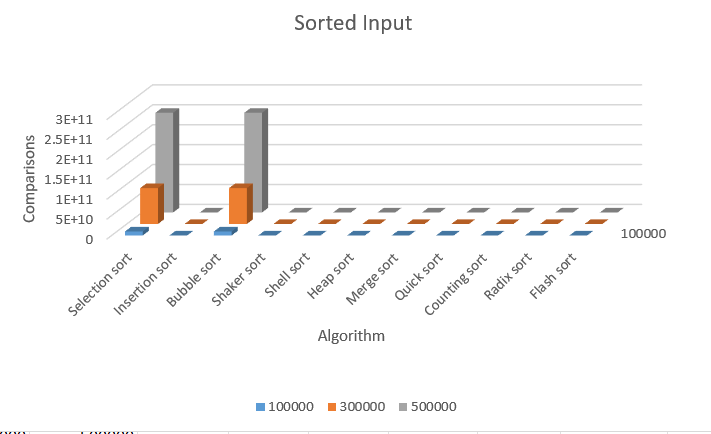
\includegraphics[scale=0.9]{BarChart2}}
\caption{Bar chart of comparisons for sorted input}
\end{figure}
\end{center}

\begin{center}
\begin{figure}[H]
\center{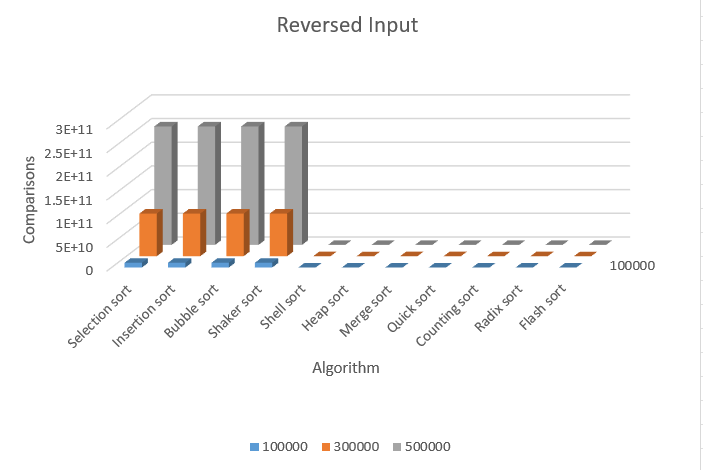
\includegraphics[scale=0.9]{BarChart3}}
\caption{Bar chart of comparisons for reversed input}
\end{figure}
\end{center}

\begin{center}
\begin{figure}[H]
\center{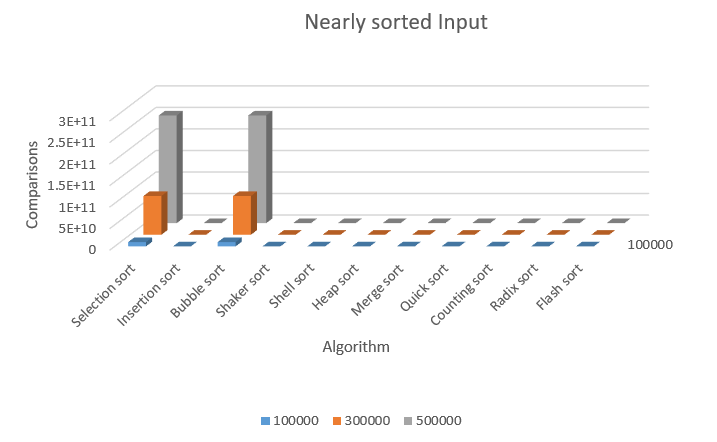
\includegraphics[scale=0.9]{BarChart4}}
\caption{Bar chart of comparisons for nearly sorted input}
\end{figure}
\end{center}

\subsection{Comments}
Due to my own observations on the graphs and charts above, I can claim that flash sort is the fastest and the most effective algorithm, because I chose $m \approx 0.43n,$ to have the best performance. Moreover, bubble sort is the slowest and the least effective in almost all cases of input because of its giant number of comparisons.\\
Besides, sorting algorithms that does not base on comparisons like counting sort, radix sort or flash sort have used less comparisons than others, significantly less.\\
It can be seen obviously that in most algorithms, sorted input will cause to least running time.\\
Here I will group algorithms due to its stability:
\begin{itemize}
 \item Stable algorithms: 
 \begin{itemize}
  \item Selection sort. It uses approximate running times with different input orders.
  \item Shell sort. I think it has shown its stability for various input orders.
  \item Heap sort. The most important part of heap sort is building a heap, which requires the same cost although there are many of input orders.
  \item Merge sort. Like heap sort, merge does the same thing for all input orders.
  \item Radix sort. On integers, I think radix sort is fine, as the experimental results have shown.
  \item Flash sort. With the complexity is approximate linear complexity, I think flash sort is an effective and stable algorithm.
  \end{itemize} 
  \item Unstable algorithms:
  \begin{itemize}
  \item Insertion sort. It has shown unefficiency when the data is reversed or randomized, meanwhile it is very fast when the data is already sorted or nearly sorted.
  \item Bubble sort. However it is always slow when the size of input is large, it has noticeably different running times for different input orders.
  \item Shaker sort. Like insertion sort, it works extremely fast when the data is sorted or nearly sorted, but has bad performance when the data is random or reversed.
  \item Quick sort. Although the graphs have shown that quicksort uses small number of comparisons and runs in a very short period of time, I will say that it is unstable, because the efficiency of this algorithm varies with the way we select the pivot, for example, if the input data is already sorted and we choose the leftmost elements of each segments to be pivots, it will be "disastrous".
  \item Counting sort. Results on these input have shown that counting sort works fast, but as I mentioned in \ref{countingsort}, it will be very uneffective when $u \gg n.$
    \end{itemize}
 \end{itemize} 
 
\section{Project organization and Programming notes}
\subsection{Project organization}
Figure below shows files in my project. 

\begin{center}
\begin{figure}[H]
\label{files}
\center{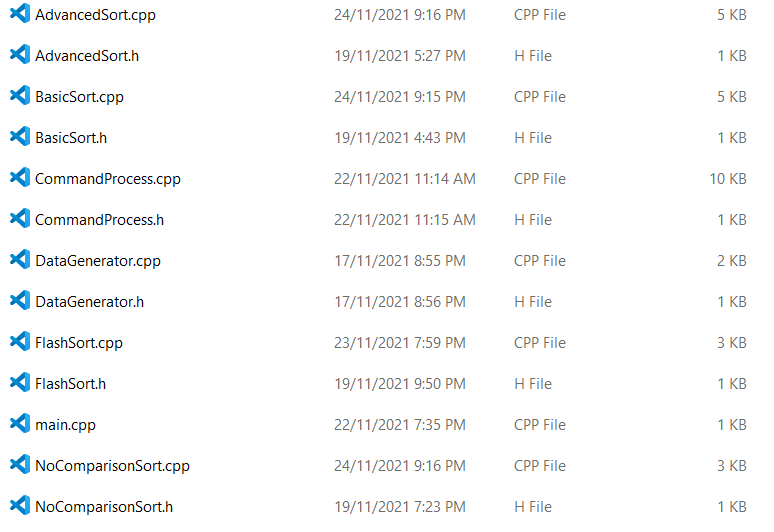
\includegraphics[scale=1]{ProjectFiles}}
\caption{Files in project}
\end{figure}
\end{center}
\begin{itemize}
\item In BasicSort files, I declared and implemented Selection sort, Insertion sort, Bubble sort, Shaker Sort, and Shell sort.
\item In AdvancedSort files, I declared and implemented Heap sort, Merge sort, and Quicksort.
\item In NoComparisonSort files, I declared and implemented Counting sort and Radix sort.
\item In FlashSort files, I spent to declare and implement Flash sort only.
\end{itemize}
\subsection{Programming notes}
My project does not use any special libraries or data structures. All are included in basic C++ 17.


\newpage
\begin{thebibliography}{9}
\bibitem{gtvlt}
Le Minh Hoang (2002) \emph{Giai thuat va lap trinh}, Ha Noi University of Education Press

\bibitem{thayP}
Lectures from Dr. Nguyen Thanh Phuong

\bibitem{sscomp}
\url{https://iq.opengenus.org/time-complexity-of-selection-sort/}

\bibitem{comp}
\url{https://www.geeksforgeeks.org/analysis-of-different-sorting-techniques}

\bibitem{bininsert}
\url{https://www.geeksforgeeks.org/binary-insertion-sort/}

\bibitem{bubble}
\url{https://www.geeksforgeeks.org/bubble-sort/}

\bibitem{shaker}
\url{https://www.javatpoint.com/cocktail-sort}

\bibitem{shaksort}
\url{https://www.geeksforgeeks.org/cocktail-sort/}

\bibitem{shell}
\url{https://www.tutorialspoint.com/Shell-Sort}

\bibitem{heap}
\url{https://www.programiz.com/dsa/heap-sort}

\bibitem{heapbuild}
\url{https://www.educative.io/blog/data-structure-heaps-guide}

\bibitem{merge}
\url{https://www.programiz.com/dsa/merge-sort}

\bibitem{quick}
\url{https://www.geeksforgeeks.org/quick-sort/}

\bibitem{itequick}
\url{https://www.geeksforgeeks.org/iterative-quick-sort/}

\bibitem{count}
\url{https://www.geeksforgeeks.org/counting-sort/}

\bibitem{counting}
\url{https://www.interviewcake.com/concept/java/counting-sort}

\bibitem{radix}
\url{https://www.geeksforgeeks.org/radix-sort/}

\bibitem{flash}
\url{https://www.w3resource.com/javascript-exercises/searching-and-sorting-algorithm/searching-and-sorting-algorithm-exercise-12.php}

\bibitem{flashsort}
\url{https://www.neubert.net/FSOIntro.html}

\end{thebibliography}
\end{document}